% Project report — compile from this folder (report/): tectonic --keep-logs main.tex
% TeX Live alternative: pdflatex main ; bibtex main ; pdflatex main ; pdflatex main
% Figures are referenced without extension: pdflatex uses figures/*.pdf (or .png); latex+dvips uses figures/*.eps.
\documentclass[12pt,a4paper]{report}
\usepackage[T1]{fontenc}
\usepackage[utf8]{inputenc}
\usepackage[a4paper,left=30mm,right=25mm,top=30mm,bottom=30mm]{geometry}
\usepackage{amsmath,amssymb,amsthm}
\usepackage{graphicx}
\usepackage{booktabs}
\usepackage{array}
\usepackage{tabularx}
\usepackage{float}
\usepackage[font=small,labelfont=bf]{caption}
\usepackage{xcolor}
\usepackage{listings}
\usepackage{setspace}
\usepackage[hidelinks]{hyperref}
\graphicspath{{figures/}}
\onehalfspacing

\newtheorem{proposition}{Proposition}[chapter]
\theoremstyle{definition}
\newtheorem{example}{Example}[chapter]
\newtheorem{definition}{Definition}[chapter]

\lstset{basicstyle=\ttfamily\scriptsize,breaklines=true,frame=single,columns=fullflexible,
        keywordstyle=\color{blue!60!black},commentstyle=\color{gray},stringstyle=\color{teal!70!black},
        language=Python,showstringspaces=false}

\newcommand{\COP}{\mathrm{COP}}
\newcommand{\kWhe}{kWh$_e$}

\begin{document}

% ------------------------------------------------------------------ title page (template layout)
\hypersetup{pageanchor=false}
\begin{titlepage}
\singlespacing
\centering
\vspace*{0.3cm}
{\large\bfseries A PROJECT REPORT\par}\vspace{0.36cm}
{\large\bfseries ON\par}\vspace{0.72cm}
{\large\bfseries Dynamic Thermal Modelling and Energy-Efficient Cooling\\ Optimization of AI Data Centres Using Optimal Control\par}
\vspace{0.84cm}
{\large BY\par}
\vspace{0.96cm}
\begin{tabular}{@{}l@{\hspace{0.8cm}}l@{\hspace{0.8cm}}l@{}}
\large Name of the student & \large ID No. & \large Discipline\\[2pt]
\large Ayush Singh  & 2023B5AD0965G & \small Mathematics and Computing\\
\large Akshat Lad   & 2023B2AD0764G & \small Mathematics and Computing\\
\large Hardik Sahu  & 2023B2AD0754G & \small Mathematics and Computing\\
\large Aarav Shah   & 2024ADPS0029G & \small Mathematics and Computing\\
\large Ayush Sanger & 2023B2AD0742G & \small Mathematics and Computing\\
\end{tabular}
\vspace{0.6cm}

{\large\bfseries Prepared in partial fulfillment of the\par}\vspace{0.15cm}
{\large\bfseries Course: Mathematical Modelling\par}\vspace{0.15cm}
{\large\bfseries MAC F314\par}
\vspace{0.6cm}
{\large AT\par}
\vspace{0.6cm}
{\large\bfseries BITS Goa\par}\vspace{0.15cm}
{\large\bfseries K K Birla Goa Campus\par}
\vspace{0.48cm}

\includegraphics[width=2.9cm]{bits_logo}\par
\vspace{0.48cm}
{\large\bfseries BIRLA INSTITUTE OF TECHNOLOGY \& SCIENCE, PILANI\par}\vspace{0.36cm}
{\large\bfseries 2026-27\par}
\end{titlepage}

% ------------------------------------------------------------------ submission page (template layout)
\thispagestyle{empty}
\begin{center}{\large\bfseries BIRLA INSTITUTE OF TECHNOLOGY \& SCIENCE, PILANI}\end{center}
\vspace{0.8cm}
\noindent
\begin{tabular}{@{}>{\bfseries}p{4.6cm}p{10.2cm}@{}}
Date of submission: & % OUTSTANDING: to be filled by the team
\\[14pt]
Title of the project: & \small Dynamic Thermal Modelling and Energy-Efficient Cooling Optimization of AI Data Centres Using Optimal Control\\[10pt]
ID No. and Name: & \small 2023B5AD0965G\quad Ayush Singh\newline 2023B2AD0764G\quad Akshat Lad\newline 2023B2AD0754G\quad Hardik Sahu\newline 2024ADPS0029G\quad Aarav Shah\newline 2023B2AD0742G\quad Ayush Sanger\\[10pt]
Discipline of the student: & \small Mathematics and Computing\\[10pt]
Course Instructor: & \small Amit Setia\\[10pt]
Keywords: & \small lumped thermal model; matrix exponential; zero-order hold; PI control; anti-windup; optimal control; linear-programming lower bound; data-centre cooling; coefficient of performance\\[10pt]
Project area(s): & \small Mathematical modelling of dynamical systems; feedback control; numerical optimisation; energy efficiency of cooling systems\\[10pt]
Acknowledgments: & % OUTSTANDING: to be written by the team (personal acknowledgements are not drafted here)
\\
\end{tabular}
\vfill
\noindent\begin{tabular}{@{}p{7.2cm}p{7.2cm}@{}}
\textbf{Signature of the student} & \textbf{Signature of the faculty member}\\[6pt]
\textbf{Date} & \textbf{Date}\\
\end{tabular}
\vspace{1.5cm}
\clearpage

\pagenumbering{arabic}
\setcounter{page}{3}
\hypersetup{pageanchor=true}
\tableofcontents
\clearpage

% ------------------------------------------------------------------ abstract
\chapter*{Abstract}
\addcontentsline{toc}{chapter}{Abstract}
Cooling an AI data hall requires balancing electricity consumption against equipment temperature limits under changing computing loads and outdoor conditions. This project investigates that trade-off using a two-node lumped thermal model of the IT equipment and room air, coupled to a chiller with a temperature-dependent coefficient of performance. The linear energy-balance equations are discretised exactly under a zero-order hold using an augmented matrix exponential. Eigenvalue analysis and closed-loop spectral radii establish model stability and guide the design of proportional--integral (PI) controllers with anti-windup.

A fixed air-temperature setpoint of 24\,\textdegree C is compared with a load-adaptive setpoint that permits warmer operation at lower IT loads. Two synthetic 17-hour scenarios test changes in IT load and outdoor temperature, with each run returning to its own initial equilibrium. Cooling electricity is evaluated from replayed trajectories, and savings are reported only when both controllers satisfy temperature limits on 5\,s and 1\,s grids and pass settling and terminal-state checks. An offline, perfect-foresight optimal-control benchmark is also computed using nonlinear optimisation, with certified linear-programming lower bounds on its discrete objective.

At 60\,s control updates, the load-adaptive strategy reduces modelled cooling electricity by 3.64\,\% in the variable-load scenario and 8.15\,\% in the outdoor-temperature scenario. These reductions agree with quasi-steady efficiency predictions and involve reduced thermal headroom during warmer operation. Sensitivity analysis shows an approximately linear energy cost for increasing the safety margin. The optimal-control benchmark derives its advantage mainly from operating closer to temperature limits; it also reveals intersample violations and discrepancies between the discrete objective and replay-integrated electricity. The results demonstrate the importance of explicit thermal margins, sufficiently frequent control updates and consistent energy accounting. All parameters are illustrative, and the numerical checks verify the implementation; validation against a real facility remains future work.

% ------------------------------------------------------------------ chapter 1
\chapter{Mathematical Methods: Linear Dynamical Models, Exact Discretisation, Feedback and Optimal Control}

\section{Literature Review}
\begin{itemize}
\item \textbf{Exact discretisation.} The project rests on standard linear systems theory. When an input is held constant over an interval (zero-order hold), a linear ODE can be discretised exactly with the matrix exponential. Van Loan~\cite{vanloan1978} showed that the integrals of matrix exponentials required for this, and for accumulated quantities such as energies, can be computed from \emph{one} exponential of an augmented block matrix.
\item \textbf{Feedback control.} PI control, closed-loop stability and integrator windup under actuator saturation are treated in \AA str\"om and Murray~\cite{astrom2021}.
\item \textbf{Optimal control.} The classical theory is introduced by Kirk~\cite{kirk2004}. Here we use the \emph{direct} approach: discretise first, then solve a finite-dimensional nonlinear program with an interior-point method (IPOPT~\cite{wachter2006}), set up through CasADi~\cite{andersson2019}.
\item \textbf{Lower bound.} The bound comes from a linear-programming relaxation solved with HiGHS~\cite{huangfu2018}. It is certified by Lagrangian weak duality~\cite{boyd2004}.
\item \textbf{Software and outlook.} The computations use NumPy~\cite{harris2020} and SciPy~\cite{virtanen2020}. Model predictive control~\cite{rawlings2017} is discussed only as future work.
\end{itemize}

\section{Mathematical Method in Our Topic}

\subsection*{Linear time-invariant model and stability}
\begin{definition}
A linear time-invariant (LTI) system is $\dot x = Ax + Bu + Ed$, with state $x\in\mathbb R^n$, control $u$ and disturbance $d$.

For constant $u,d$, an equilibrium $x^\ast$ solves $Ax^\ast=-(Bu+Ed)$. It is asymptotically stable if every eigenvalue of $A$ has a negative real part, and the time constants are $\tau_i=-1/\lambda_i$.
\end{definition}

\begin{proposition}\label{prop:sym}
If $A=D^{-1}SD$ with $D$ diagonal positive and $S$ symmetric, then all eigenvalues of $A$ are real.
\end{proposition}
\noindent\emph{Proof.} $A$ is similar to the symmetric $S$, and similar matrices have the same eigenvalues. \hfill$\square$

\noindent For our thermal model, $D=\mathrm{diag}(\sqrt{C_s},\sqrt{C_a})$ does this. Physically, the model cannot oscillate on its own.

\subsection*{Exact zero-order-hold discretisation}
\begin{proposition}[Exact discretisation~\cite{vanloan1978}]\label{prop:zoh}
Let $\dot X=FX+Hw$ with $w$ constant on $[t,t+h)$. Then $X(t+h)=\Phi X(t)+\Gamma w$, where $\Phi=e^{Fh}$ and $\Gamma=\int_0^h e^{Fs}\,ds\,H$. Moreover,
\[
\exp\!\left(\begin{bmatrix}F&H\\0&0\end{bmatrix}h\right)=\begin{bmatrix}\Phi&\Gamma\\0&I\end{bmatrix}.
\]
\end{proposition}
\noindent\emph{Proof sketch.} The augmented system $\frac{d}{dt}[X;w]=\begin{bmatrix}F&H\\0&0\end{bmatrix}[X;w]$ keeps $w$ constant. Its exact solution over a time $h$ is the exponential of the block matrix. Comparing the blocks with the variation-of-constants formula $X(t+h)=e^{Fh}X(t)+\int_0^h e^{Fs}\,ds\,Hw$ gives the result. \hfill$\square$

\noindent \textbf{How we use it.} We append the running integrals of heat removed, IT heat and envelope heat to $X$, so energy totals are propagated exactly together with the temperatures. There is \emph{no} time-step error, unlike forward Euler, which is unstable for $h>2\tau_{\min}$.

\subsection*{Discrete PI feedback with anti-windup}
At updates $t_k=k\,\Delta t$ the controller measures $T_{a,k}$ and computes $e_k=T_{a,k}-T_{set}$, $I_k=I_{k-1}+K_i\Delta t\,e_k$ and $u_k=\mathrm{sat}_{[0,u_{\max}]}(K_pe_k+I_k)$. The command is held until $t_{k+1}$.

\begin{itemize}
\item \textbf{Closed loop without saturation.} With $z_k=[x_k;I_{k-1}]$, the loop is linear, $z_{k+1}=Mz_k$ (plus constant terms), where
\[
M=\begin{bmatrix}\Phi+(K_p+K_i\Delta t)\Gamma_u c&\Gamma_u\\K_i\Delta t\,c&1\end{bmatrix},\qquad c=[0\;\;1].
\]
It is asymptotically stable if and only if the spectral radius $\rho(M)<1$.
\item \textbf{Gain design.} We choose $(K_p,K_i)$ on a grid to minimise $\rho(M)$, subject to $\rho<1$ also at twice the gains (a robustness margin).
\item \textbf{Anti-windup (conditional integration).} If an update would push the command further past a limit, the integrator is advanced only up to that limit~\cite{astrom2021}:
\begin{itemize}
\item at the upper limit, $I_k=\max(I_{k-1},u_{\max}-K_pe_k)$;
\item at the lower limit, $I_k=\min(I_{k-1},-K_pe_k)$.
\end{itemize}
\end{itemize}

\subsection*{Discrete optimal control and a certified lower bound}
\begin{itemize}
\item \textbf{The problem.} We minimise $J_d(u,x)=\sum_k \Delta t\,u_k\,g(x_k,d_k)$ subject to the exact discrete dynamics $x_{k+1}=\Phi x_k+\Gamma[u_k;d_k]$, box bounds, state bounds at the sample points, and $x_0=x_N=x_{start}$. Here $g=1/\COP$.
\item \textbf{The solver.} This is a sparse nonlinear program, solved by a primal--dual interior-point method~\cite{wachter2006}. It returns a local (KKT) point; from several starts we report the \emph{best-found} value, not a proven global optimum.
\item \textbf{The lower bound.} If $g(x,d)\ge \underline g(d)$ for every feasible $x$, and every feasible $u_k\ge0$, then the LP with cost $\sum_k\Delta t\,u_k\,\underline g(d_k)$ and the same constraints has optimum $J_{LB}\le J_d^\ast$.
\end{itemize}

\begin{proposition}[Weak duality~\cite{boyd2004}]\label{prop:wd}
For the LP $\min\{c^\top z: Az=b,\ l\le z\le u\}$ and \emph{any} vector $y$,
\[
c^\top z\ \ge\ b^\top y+\sum_i\min(r_il_i,\ r_iu_i)\qquad\text{for every feasible }z,\qquad r=c-A^\top y.
\]
\end{proposition}
\noindent\emph{Proof.} $c^\top z=r^\top z+y^\top Az=r^\top z+y^\top b$, and $r_iz_i\ge\min(r_il_i,r_iu_i)$ for $l_i\le z_i\le u_i$. \hfill$\square$

\noindent \textbf{Why this matters.} Evaluating the right-hand side with the solver's multipliers gives a lower bound that we verify ourselves, whatever status message the solver reports. The gap $(J_d(\text{best})-J_{LB})/J_{LB}$ bounds suboptimality \emph{in $J_d$ only}.

\section{Examples of the Mathematical Method}

\begin{example}[Exact discretisation versus Euler for a scalar mode]\label{ex:zoh}
Take $\dot T=-a\,T+b\,u$ with $u$ held constant over a step $h$. Proposition~\ref{prop:zoh} with $F=-a$, $H=b$ gives
\[
\Phi=e^{-ah},\qquad \Gamma=\int_0^h e^{-as}\,ds\;b=\frac{1-e^{-ah}}{a}\,b .
\]
In our model the fast (air) mode has $a\approx(UA_s+UA_e)/C_a=68\,667/3\,618\,000=0.018979\ \mathrm{s^{-1}}$, i.e.\ $1/a=52.7$\,s.
\begin{itemize}
\item For $h=5,60,300$\,s, $\Phi=0.9095,\ 0.3202,\ 0.0034$: always in $(0,1)$, so the exact map is stable for every $h$.
\item Forward Euler uses $\Phi_E=1-ah$, which gives $-0.139$ at $h=60$\,s and $-4.69$ at $h=300$\,s. For $h>2/a\approx105$\,s, $|1-ah|>1$ and Euler is unstable.
\end{itemize}
For the full 2-state model the Euler limit is $2\tau_{fast}=92.7$\,s. This is why the project propagates exactly.
\end{example}

\begin{example}[Eigenvalues, time constants and an equilibrium of the thermal model]\label{ex:eig}
With $C_s=2.5\times10^7$\,J/K, $C_a=3.618\times10^6$\,J/K, $UA_s=66\,667$\,W/K and $UA_e=2000$\,W/K,
\[
A=\begin{bmatrix}-0.0026667&0.0026667\\0.0184264&-0.0189792\end{bmatrix}\ \mathrm{s^{-1}}.
\]
\begin{itemize}
\item $\operatorname{tr}A=-0.0216458$ and $\det A=1.47411\times10^{-6}$, so
\[
\begin{aligned}
\lambda&=\tfrac12\big(\operatorname{tr}A\pm\sqrt{(\operatorname{tr}A)^2-4\det A}\big)\\
&=-0.0215775,\ -6.8317\times10^{-5}\ \mathrm{s^{-1}}.
\end{aligned}
\]
\item Both eigenvalues are real (Proposition~\ref{prop:sym}) and negative. The time constants are $\tau_{fast}=46.3$\,s (air) and $\tau_{slow}=14\,638$\,s $=4.07$\,h (equipment).
\item \textbf{Equilibrium.} Hold the air at $T_a=24$\,\textdegree C with $P_{IT}=0.6$\,MW and $T_{out}=30$\,\textdegree C. Setting $\dot x=0$ gives the holding cooling
\[
Q_c=P_{IT}+UA_e(T_{out}-T_a)=600\,000+2000\times 6=612\ \mathrm{kW_{th}},
\]
and the equipment temperature $T_s=T_a+P_{IT}/UA_s=24+9=33$\,\textdegree C.
\item With
\[
\COP(24,30)=0.45\times285.15/(311.15-285.15)=4.935,
\]
this costs $612/4.935=124.0$\,kW$_e$. Holding 26\,\textdegree C instead needs $Q_c=608$\,kW$_{th}$ at $\COP=5.384$, i.e.\ $112.9$\,kW$_e$: 8.9\,\% less electricity.
\end{itemize}
\end{example}

\begin{example}[Weak-duality bound on a two-interval toy problem]\label{ex:wd}
Remove 1 unit of heat over two intervals with costs $c=(0.2026,\ 0.1774)$, i.e.\ $1/\COP$ at 24 and 27\,\textdegree C: $\min c_1u_1+c_2u_2$ subject to $u_1+u_2=1$, $0\le u\le1$. The optimum is $0.1774$, putting all the heat in the cheaper interval. Proposition~\ref{prop:wd} gives, for any $y$:
\begin{itemize}
\item $y=0.1774$: $r=(0.0252,0)$, so the bound is $0.1774+0+0=0.1774$ (tight).
\item $y=0.19$: $r=(0.0126,-0.0126)$, so the bound is $0.19+0-0.0126=0.1774$.
\item $y=0.25$: $r=(-0.0474,-0.0726)$, so the bound is $0.25-0.0474-0.0726=0.13$. This is valid, but loose.
\end{itemize}
Every $y$ gives a valid lower bound, and the best $y$ certifies optimality. In the project the same formula is applied to LPs with up to about 25\,000 constraints. The finite lower bounds on the equipment temperature that the formula needs are derived from the dynamics.
\end{example}

% ------------------------------------------------------------------ chapter 2
\chapter{An Application of the Mathematical Method: Cooling an AI Data Hall}

\section{Literature Review: Introduction to the Problem}
\begin{itemize}
\item \textbf{The problem.} Almost all of a data hall's IT electricity ends up as heat, which the cooling plant must remove. The electricity this costs is not fixed: a vapour-compression chiller's coefficient of performance (COP) depends on the temperatures it works between, and it improves when the room air is warmer.
\item \textbf{Why it matters for AI halls.} The IT load changes with the workload, so a cooling setpoint chosen to be safe at peak load may be colder than necessary most of the time.
\item \textbf{Our question.} Within a transparent model, how much cooling electricity does a warmer or load-dependent setpoint save, how much does an idealised optimal schedule save, and what thermal safety margin does each give up?
\end{itemize}
This is a modelling study with \emph{illustrative} parameters (plausible orders of magnitude, not measured values). It is not a study of a particular facility.

\section{Where and Why the Methods Are Used}
\begin{itemize}
\item \textbf{The model} is a two-state LTI system (Chapter~1), simple enough to analyse by hand and to explain fully. Its eigenvalues show two time scales: 46\,s for the air and 4.07\,h for the equipment (Example~\ref{ex:eig}). These explain why a 5-minute controller update can miss fast air excursions.
\item \textbf{Exact ZOH propagation} (Proposition~\ref{prop:zoh}) matches how a digital controller works, holding its command between updates. It also gives exact energy totals.
\item \textbf{The PI controller} is the standard industrial baseline, and its stability can be checked exactly through $\rho(M)$.
\item \textbf{The optimal-control problem} answers ``what could perfect foresight achieve in this model?''. The LP bound tells us how far the best-found answer could be from the true optimum of that discrete problem.
\end{itemize}

\section{Methodology}

\subsection*{Model}
Energy balances on the equipment mass and the room-air mass (Figure~\ref{fig:diagram}) give
\[
C_s\dot T_s=P_{IT}-UA_s(T_s-T_a),\qquad C_a\dot T_a=UA_s(T_s-T_a)+UA_e(T_{out}-T_a)-Q_c .
\]
Integrating the total stored heat $U=C_sT_s+C_aT_a$ gives $E_Q=E_{IT}+E_{env}-\Delta U$. Over a closed cycle ($\Delta U=0$) the heat removed equals the heat released plus the heat leaked in.

\noindent\textbf{Cooling electricity.} With a Carnot-fraction chiller (temperatures in kelvin),
\[
\begin{gathered}
\COP=\eta_{II}\frac{T_{ev}}{T_{cd}-T_{ev}},\quad T_{ev}=T_a-12,\quad T_{cd}=T_{out}+8,\\
E_{cool}=\int_0^{t_f}\frac{Q_c}{\COP(T_a,T_{out})}\,dt .
\end{gathered}
\]
$E_{cool}$ is integrated by Simpson's rule on 5\,s segments, using exactly propagated midpoints. The model is used only where the lift is positive and $\COP\le10$; elsewhere the simulation stops instead of extrapolating. The parameters are listed in Table~\ref{tab:params}.

\begin{figure}[H]
\centering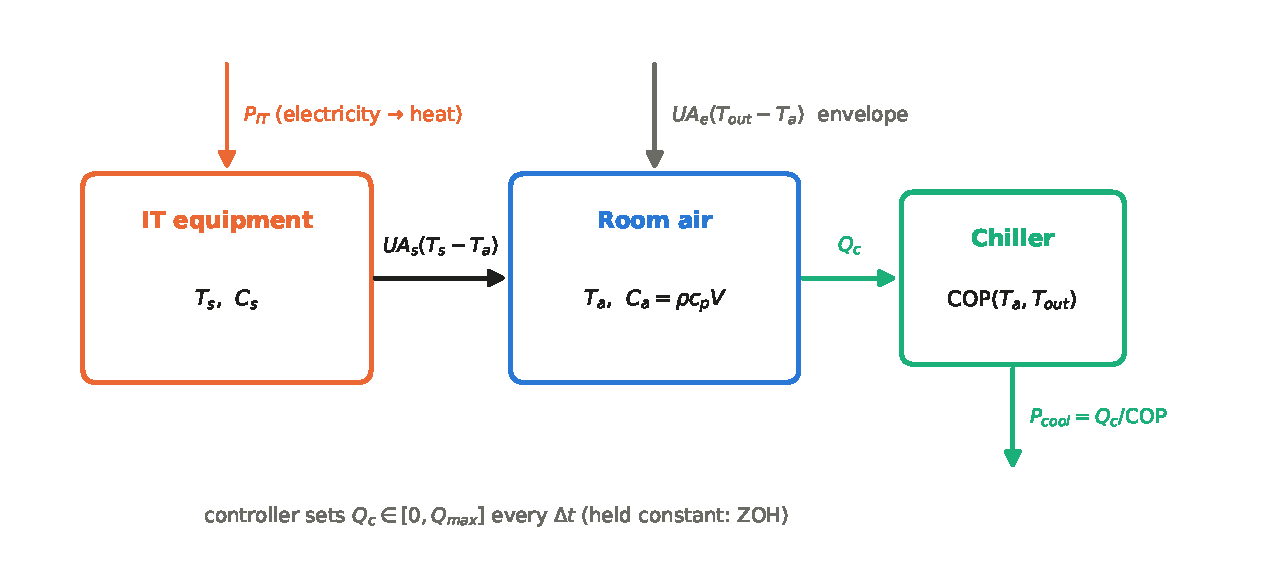
\includegraphics[width=0.92\textwidth]{fig1_model_diagram}
\caption{Two-node lumped model. Heat flows (W$_{th}$) are shown in the colours of the nodes they connect; the controller sets $Q_c$ every $\Delta t$ and holds it constant (ZOH). Diagram drawn from code in \texttt{notebook/main.ipynb}.}
\label{fig:diagram}
\end{figure}

\begin{table}[H]
\centering\small
\caption{Model parameters. [ILL] = illustrative (not measured, not calibrated); [STD] = standard constant.}
\label{tab:params}
\begin{tabularx}{\textwidth}{@{}lXll@{}}
\toprule
Symbol & Meaning & Value & Tag\\
\midrule
$C_a=\rho c_pV$ & air heat capacity ($1.2\times1005\times3000$) & $3.618\times10^6$ J/K & STD/ILL\\
$C_s$ & lumped IT-equipment heat capacity & $2.5\times10^7$ J/K & ILL\\
$UA_s$ & equipment-to-air conductance (15 K rise at 1 MW) & $66\,667$ W/K & ILL\\
$UA_e$ & envelope conductance & $2000$ W/K & ILL\\
$Q_{\max}$ & cooling capacity & 1.5 MW$_{th}$ & ILL\\
$\eta_{II}$, $\Delta T_{ev}$, $\Delta T_{cd}$ & Carnot fraction; heat-exchanger approaches & 0.45; 12 K; 8 K & ILL\\
limits & air 18--27\,\textdegree C; lumped equipment $\le$ 40\,\textdegree C & -- & ILL\\
\bottomrule
\end{tabularx}
\end{table}

\subsection*{Controllers}
\begin{itemize}
\item \textbf{B1 (fixed-setpoint PI).} $T_{set}=\min(27,\,40-P_{IT,\max}/UA_s)-m=24$\,\textdegree C, with margin $m=1$\,K and peak load 1\,MW.
\item \textbf{B2 (load-adaptive PI).} The same PI law, gains and anti-windup, but the setpoint is recomputed at each update from the measured load:
\[
T_{set}=\mathrm{clip}(\min(27,\,40-P_{IT}/UA_s)-m,\,18,\,27).
\]
This gives 26\,\textdegree C at 0.6 and 0.8\,MW, and 24\,\textdegree C at 1.0\,MW.
\item \textbf{Gains.} They were designed for \emph{stability}, by minimising $\rho(M)$ with a $2\times$ gain margin, separately for $\Delta t=60$\,s and $300$\,s. Their spectral radii are $0.686$ and $0.565$. They were not tuned for energy.
\end{itemize}

\subsection*{Optimal-control benchmark (OC)}
\begin{itemize}
\item \textbf{The problem $\mathcal P_d$.} The variables are the commands and the states on the update grid; the dynamics are the exact discrete ones. The limits are imposed at the sample points, with $x_0=x_N$ equal to the matched PI controller's own start state (the \emph{boundary protocol}: B1 or B2). The objective is $J_d$ (Chapter~1) with $g=1/\COP$ evaluated at the start of each interval.
\item \textbf{Variant OC-ISC5.} It also imposes the limits every 5\,s inside each interval; these constraints remain linear.
\item \textbf{Solving and the bound.} IPOPT via CasADi is run from four starts (the matched PI warm start and three seeded perturbations). The LP lower bound uses $\underline g=1/\COP(27\,^\circ\mathrm{C},T_{out})$, which is valid because $\partial g/\partial T_a=-T_{cd}/(\eta_{II}T_{ev}^2)<0$.
\item \textbf{Status.} The OC benchmark is offline (it knows the future), uses perfect foresight and is best-found. It is not a deployable controller.
\end{itemize}

\subsection*{Scenarios and evaluation protocol}
\begin{itemize}
\item \textbf{Scenarios.} There are two synthetic 17\,h closed-cycle step scenarios, defined in code; no measured data are used.
\begin{itemize}
\item \textbf{S1:} the load steps 0.6$\to$1.0\,MW at 1\,h and back to 0.6\,MW at 9\,h, with $T_{out}=30$\,\textdegree C.
\item \textbf{S2c:} the load stays at 0.8\,MW and $T_{out}$ steps 30$\to$35\,\textdegree C at 1\,h and back at 9\,h.
\end{itemize}
\item \textbf{Own-equilibrium closed cycles.} Each run starts at its \emph{own} equilibrium, at its own setpoint and the starting load. It must return to that state by the end ($|\Delta T|\le10^{-3}$\,K and negligible $\Delta U$). Initial states therefore differ between controllers.
\item \textbf{Two replay grids.} Every run, including the OC command sequences, is replayed through the same plant on 5\,s and 1\,s grids. Energy is always the replay-integrated $E_{cool}$, never $J_d$.
\item \textbf{Strict eligibility.} A saving is claimed only when \emph{both} compared runs:
\begin{itemize}
\item are complete;
\item stay within the limits on the 5\,s \emph{and} the 1\,s grid;
\item settle within $\pm0.1$\,K of their setpoint (PI);
\item pass the terminal checks.
\end{itemize}
\end{itemize}

\section{Numerical Demonstration and Results}

\subsection*{Fixed versus load-adaptive PI}
Before any simulation, a quasi-steady COP calculation (as in Example~\ref{ex:eig}) predicted savings of 3.62\,\% (S1) and 8.15\,\% (S2c). Table~\ref{tab:pi} and Figure~\ref{fig:pi} show the simulated results.

\begin{table}[H]
\centering\small
\caption{Cooling electricity over 17\,h, B1 (24\,\textdegree C) versus B2 ($m=1$\,K). Model results, illustrative parameters.}
\label{tab:pi}
\begin{tabularx}{\textwidth}{@{}lrrrr>{\raggedright\arraybackslash}X@{}}
\toprule
Case & $E_{B1}$ (\kWhe) & $E_{B2}$ (\kWhe) & Saving & Predicted & Status\\
\midrule
S1, 60\,s  & 2756.5 & 2656.2 & +3.64\,\% & +3.62\,\% & both eligible\\
S1, 300\,s & 2756.7 & 2656.2 & n/a & +3.62\,\% & B1 unsafe: $T_a$ reaches 27.44\,\textdegree C\\
S2c, 60\,s & 3069.4 & 2819.3 & +8.15\,\% & +8.15\,\% & both eligible\\
S2c, 300\,s & 3069.4 & 2819.3 & +8.15\,\% & +8.15\,\% & both eligible\\
\bottomrule
\end{tabularx}
\end{table}

\begin{figure}[H]
\centering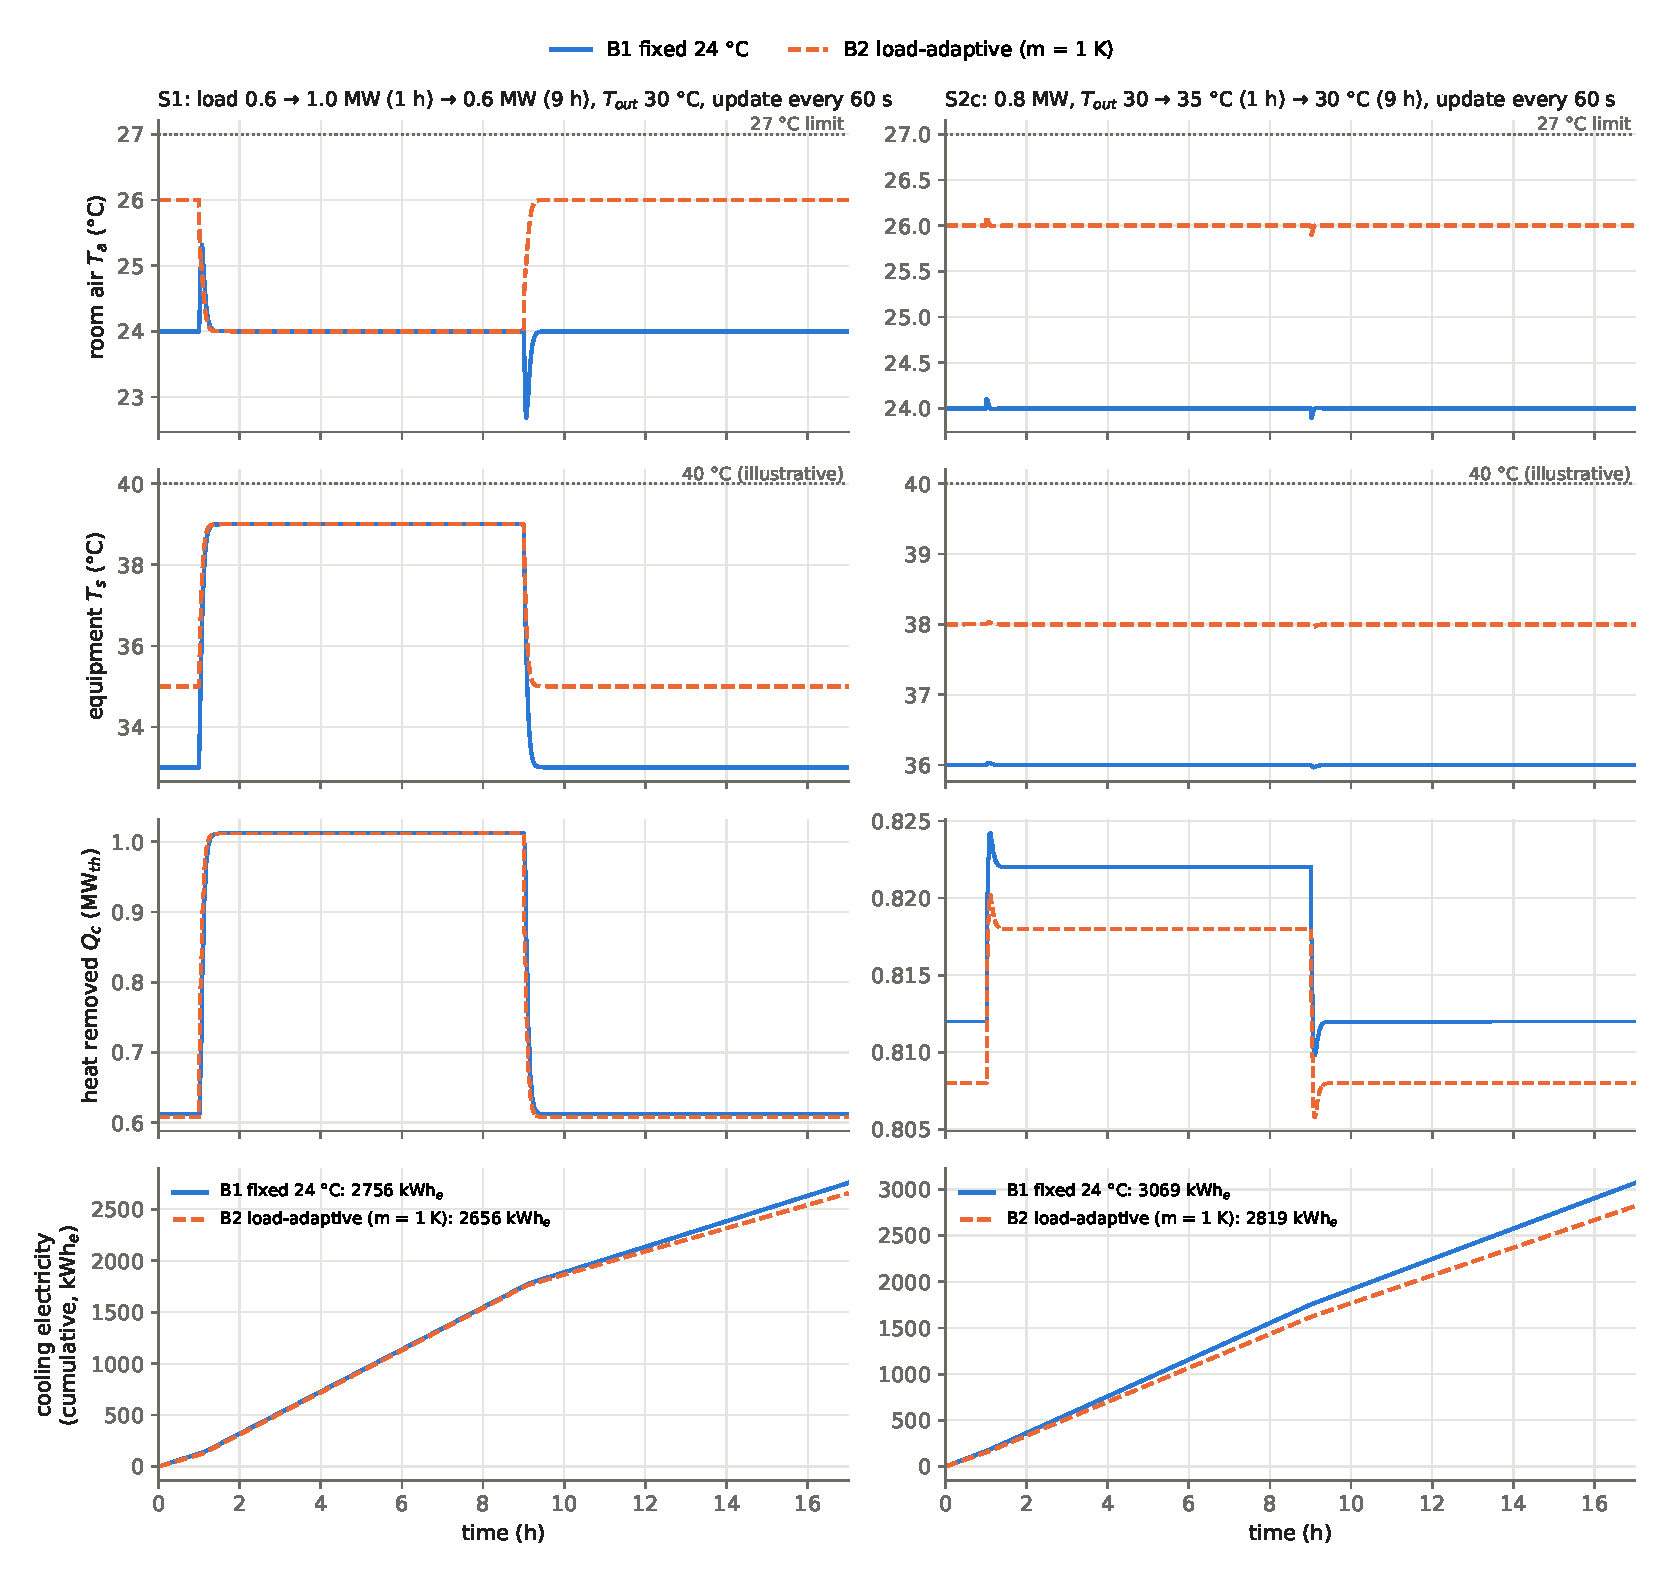
\includegraphics[width=\textwidth]{fig2_b1_b2_60s}
\caption{B1 (fixed 24\,\textdegree C) and B2 (load-adaptive) at 60\,s updates. Left: S1; right: S2c. B2 runs the air 2\,K warmer whenever the load is below 1\,MW, and its equipment correspondingly runs 2\,K closer to the illustrative 40\,\textdegree C limit.}
\label{fig:pi}
\end{figure}

\noindent\textbf{Reading the comparison.}
\begin{itemize}
\item \textbf{The saving is quasi-steady.} The measured and predicted savings agree to within 0.02 percentage points, so the saving comes from steady-state COP and is not a transient effect.
\item \textbf{The cost.} At 0.8\,MW, B2 holds the lumped equipment at 38\,\textdegree C against B1's 36\,\textdegree C.
\item \textbf{S1 at 300\,s.} The fixed-setpoint baseline exceeds 27\,\textdegree C after the load step, so no saving is claimed there.
\end{itemize}

\subsection*{Optimal-control benchmark}
Table~\ref{tab:oc} compares OC with B2 under the B2 boundary protocol.

\begin{table}[H]
\centering\footnotesize
\caption{OC (offline, perfect foresight, best-found) versus B2 PI, both starting and ending at B2's equilibrium. $E$: replayed cooling electricity (\kWhe). $J_d$: the optimiser's discrete objective. The LP gap concerns $J_d$ only. ``Max.\ exceed.'' is the largest limit exceedance on the finer grid where it occurs.}
\label{tab:oc}
\setlength{\tabcolsep}{3pt}
\begin{tabularx}{\textwidth}{@{}llrrrrrrX@{}}
\toprule
Case & Variant & $E_{B2}$ & $E_{OC}$ & Saving & $J_{d}$ & $J_{LB}$ & Gap & Status / max.\ exceedance\\
\midrule
S1, 300\,s & OC      & 2656.2 & 2535.5 & n/a & 2535.0 & 2400.6 & 5.60\,\% & unsafe: 0.652\,K (5\,s grid)\\
S1, 300\,s & OC-ISC5 & 2656.2 & 2536.3 & n/a & 2535.9 & 2400.7 & 5.63\,\% & diagnostic: $4.8\times10^{-5}$\,K (1\,s grid)\\
S1, 60\,s  & OC      & 2656.2 & 2554.9 & n/a & 2500.1 & 2400.6 & 4.15\,\% & unsafe: 0.079\,K (5\,s grid)\\
S1, 60\,s  & OC-ISC5 & 2656.2 & 2550.4 & n/a & 2502.6 & 2400.6 & 4.25\,\% & diagnostic: $7.5\times10^{-4}$\,K (1\,s grid)\\
S2c, 300\,s & both   & 2819.3 & 2698.2 & +4.29\,\% & 2698.1 & 2694.9 & 0.12\,\% & eligible\\
S2c, 60\,s  & both   & 2819.3 & 2697.6 & +4.32\,\% & 2697.1 & 2694.6 & 0.09\,\% & eligible\\
\bottomrule
\end{tabularx}
\end{table}

\noindent\textbf{Reading the OC results} (Table~\ref{tab:oc} and Figure~\ref{fig:oc}):
\begin{itemize}
\item \textbf{OC removes the margin.} It holds the air at exactly 27\,\textdegree C, or, at 1\,MW, the equipment at 40\,\textdegree C. A quasi-steady estimate at those limit temperatures lies within a few \kWhe\ of the 300\,s OC results. So OC's advantage over B2 is essentially the energy cost of B2's 1\,K margin, not clever timing.
\item \textbf{Against B1.} Under the B1 boundary protocol, OC saves about 12\,\% in S2c. That figure mostly reflects B1's cold fixed setpoint.
\item \textbf{Sample points are not enough.} In S1, the basic OC is feasible at every update but exceeds the limits \emph{between} updates (Figure~\ref{fig:oc}b).
\item \textbf{OC-ISC5 is only diagnostic in S1.} It removes the exceedance on the 5\,s grid, but still exceeds by up to $4.8\times10^{-5}$\,K (300\,s) and $7.5\times10^{-4}$\,K (60\,s) on the 1\,s grid. These S1 results are therefore \emph{diagnostic only}: they are not continuously safe and not eligible under the strict rule.
\item \textbf{$J_d$ under-counts electricity at 60\,s.} The optimiser switches cooling every minute (Figure~\ref{fig:oc}c). $J_d$ charges each minute at the COP of its starting temperature, so in S1 it lies about 48--56\,\kWhe\ below the replayed electricity. The switching also raises peak cooling power to roughly 350--380\,kW$_e$, against about 205--210\,kW$_e$ for PI.
\item \textbf{What the LP gap means.} The certified gap is 0.09--0.24\,\% in S2c but 4.1--5.7\,\% in S1, where the bound is loose: it charges COP at 27\,\textdegree C, while at 1\,MW the equipment limit keeps the air near 25\,\textdegree C. The gap says nothing about continuous-time electricity or global optimality.
\end{itemize}

\begin{figure}[H]
\centering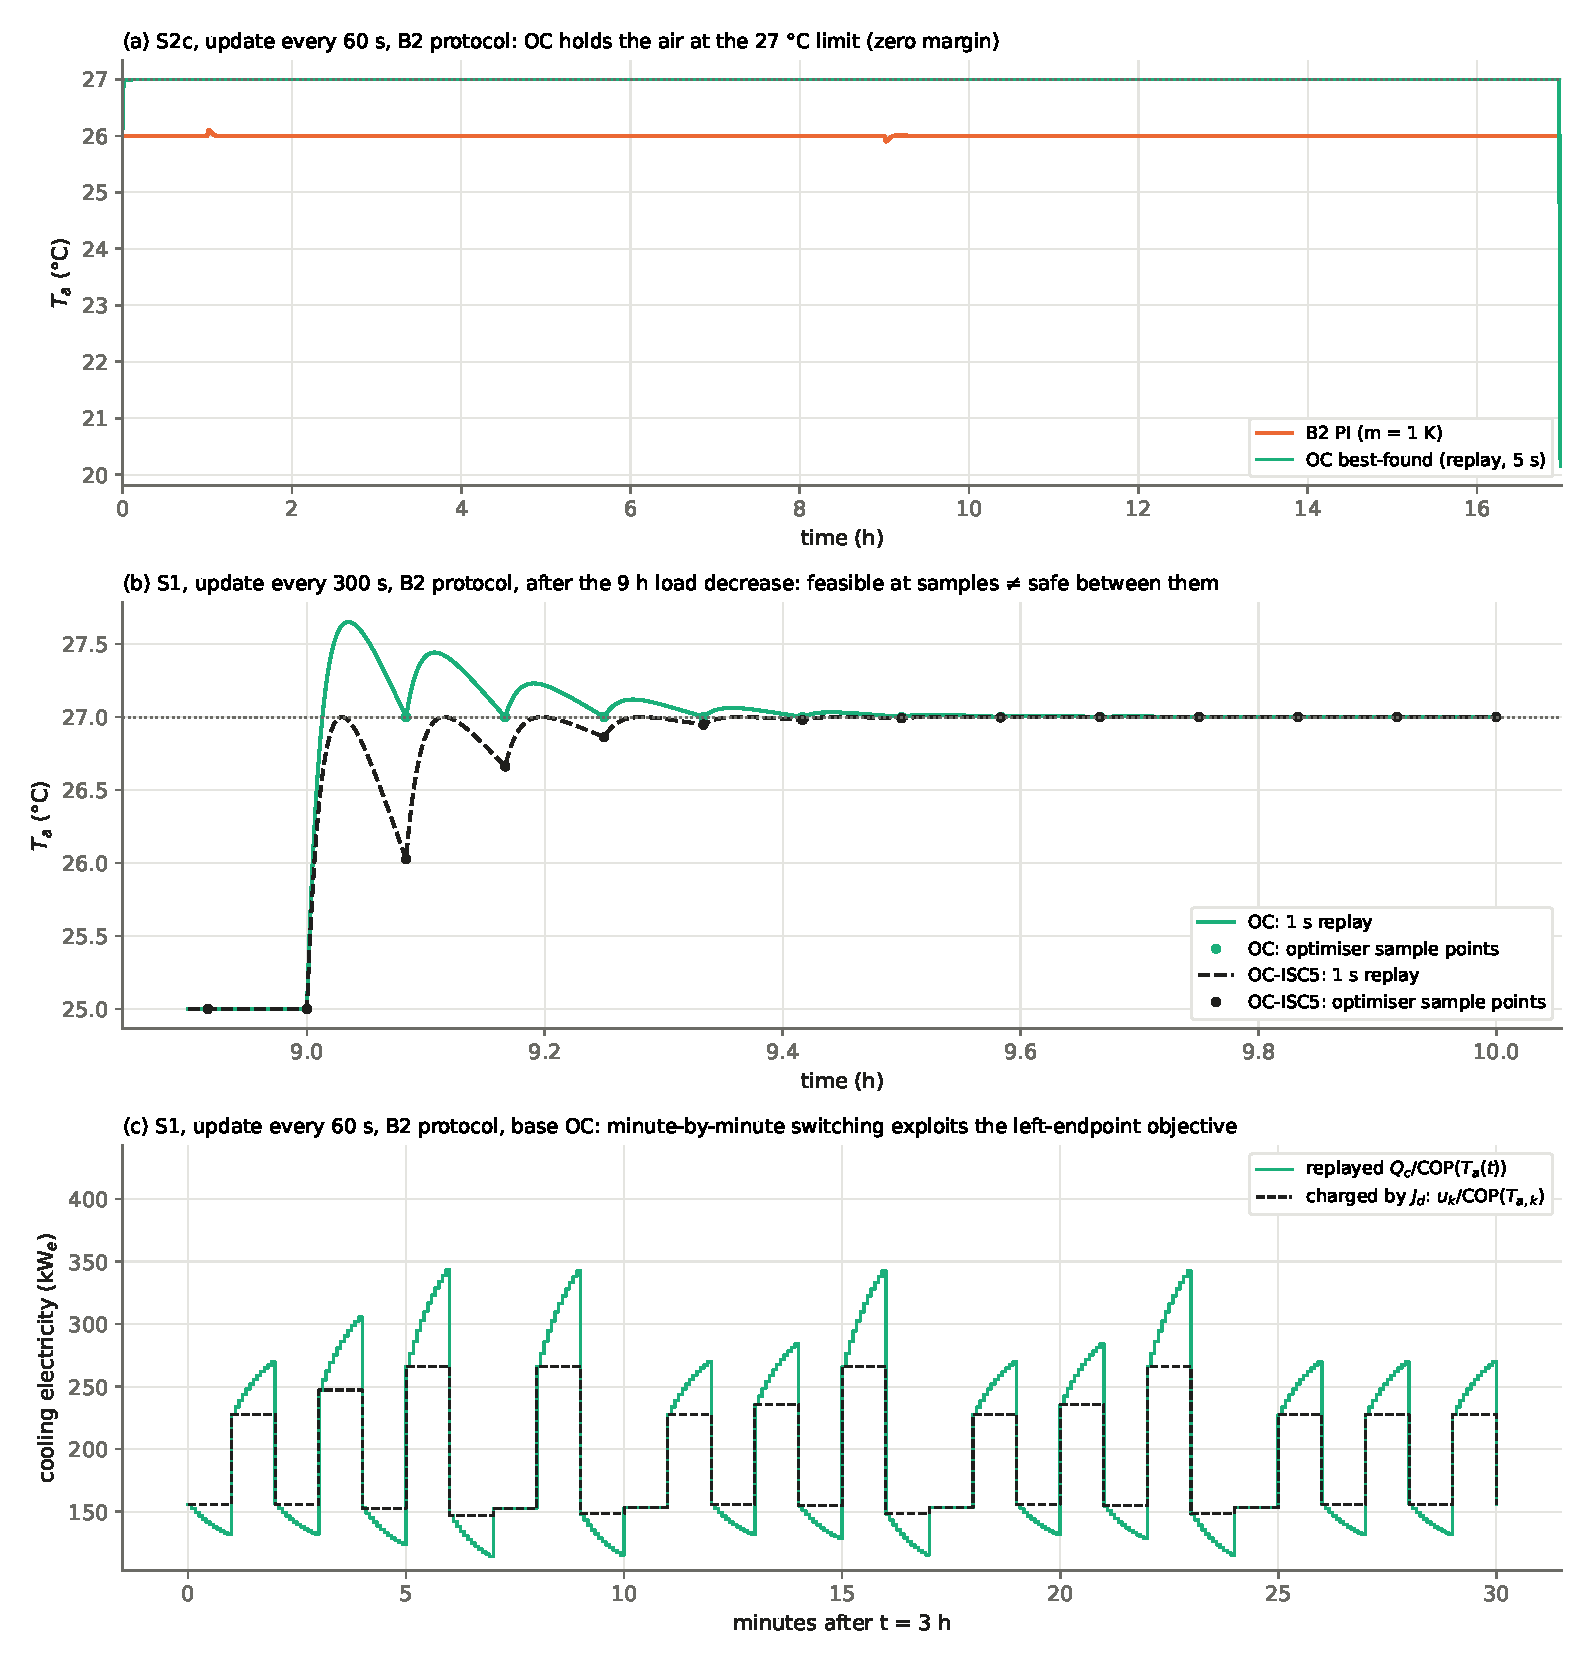
\includegraphics[width=0.93\textwidth]{fig3_oc_benchmark}
\caption{OC benchmark, B2 protocol. (a) S2c, 60\,s: OC holds the air at the 27\,\textdegree C limit; the drop in the final minutes is the forced return to B2's start state (closed cycle), still above 18\,\textdegree C. (b) S1, 300\,s, after the 9\,h load decrease (1\,s replay): OC is feasible at the sample points but overshoots 27\,\textdegree C between them. OC-ISC5 stays within the limit on the 5\,s grid, but on this 1\,s grid exceeds it by up to $4.8\times10^{-5}$\,K (invisible at this scale). (c) S1, 60\,s: replayed electricity versus what the discrete objective $J_d$ charges, during minute-by-minute switching.}
\label{fig:oc}
\end{figure}

\subsection*{Sensitivity to the safety margin and the fixed setpoint}
Table~\ref{tab:sens} and Figure~\ref{fig:sens} sweep B2's margin $m$ and B1's setpoint. The gains are unchanged, and the strict eligibility rule applies.

\begin{table}[H]
\centering\small
\caption{Sensitivity at 60\,s updates: cooling electricity (\kWhe), saving versus B1 at 24\,\textdegree C, and worst-case headroom to the limits on the 1\,s grid (K). All runs eligible.}
\label{tab:sens}
\begin{tabular}{@{}lrrrrrr@{}}
\toprule
 & \multicolumn{3}{c}{S1} & \multicolumn{3}{c}{S2c}\\
\cmidrule(lr){2-4}\cmidrule(l){5-7}
Controller & $E$ & Saving & Headroom & $E$ & Saving & Headroom\\
\midrule
B2, $m=0.5$ K & 2595.8 & +5.83\,\% & 0.50 & 2757.6 & +10.16\,\% & 0.40\\
B2, $m=1$ K   & 2656.2 & +3.64\,\% & 1.00 & 2819.3 & +8.15\,\%  & 0.90\\
B2, $m=1.5$ K & 2717.1 & +1.43\,\% & 1.50 & 2881.3 & +6.13\,\%  & 1.40\\
B2, $m=2$ K   & 2778.2 & $-0.79$\,\% & 2.00 & 2943.7 & +4.10\,\% & 1.90\\
B1, 23\,\textdegree C & 2879.7 & $-4.47$\,\% & 2.00 & 3196.6 & $-4.14$\,\% & 3.90\\
B1, 24\,\textdegree C & 2756.5 & baseline & 1.00 & 3069.4 & baseline & 2.90\\
B1, 25\,\textdegree C & 2634.6 & +4.42\,\% & 0.00 & 2943.7 & +4.10\,\% & 1.90\\
\bottomrule
\end{tabular}
\end{table}

\begin{figure}[H]
\centering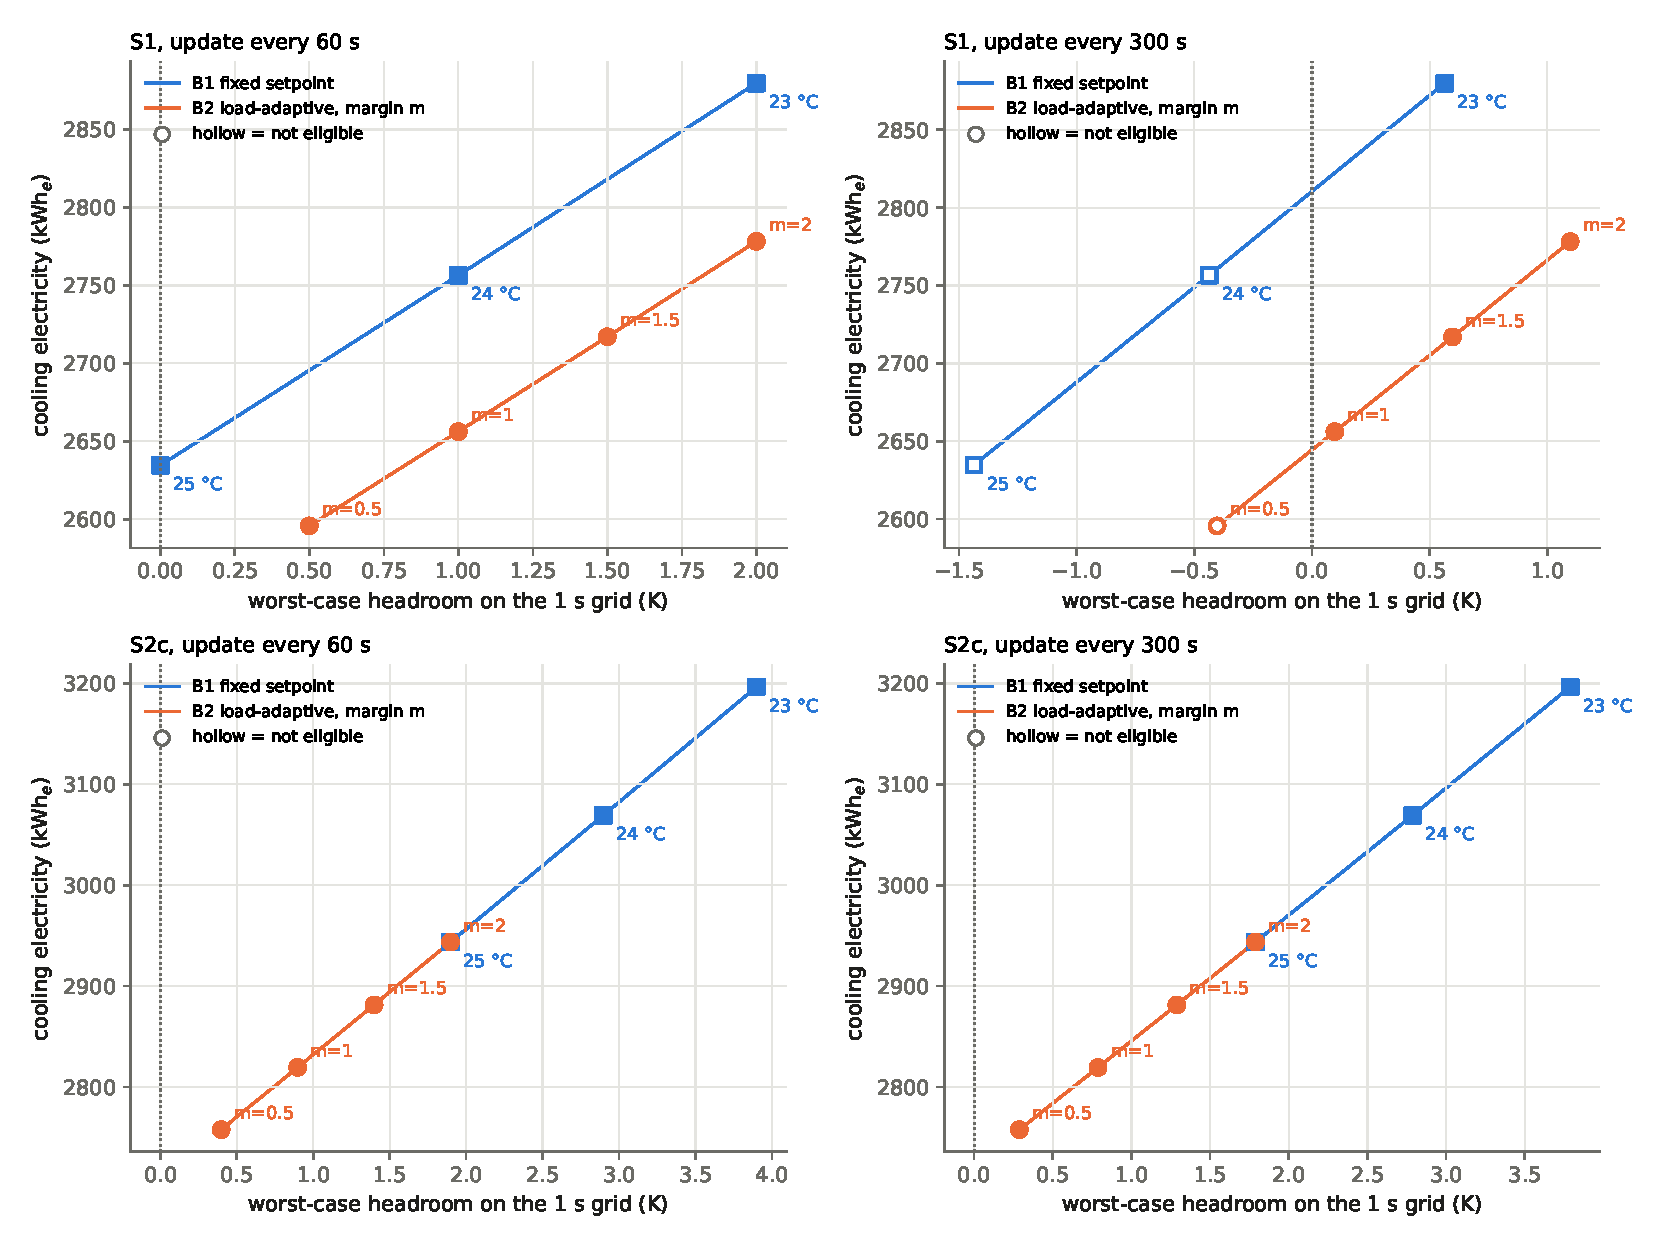
\includegraphics[width=0.95\textwidth]{fig4_sensitivity}
\caption{Cooling electricity versus worst-case headroom (1\,s grid) for the B2 margin sweep and the B1 setpoint sweep. Hollow markers are not eligible (unsafe). The OC results are not shown, because their start and end states differ.}
\label{fig:sens}
\end{figure}

\noindent\textbf{Reading the sensitivity sweep.}
\begin{itemize}
\item \textbf{Margin costs energy steadily.} Each extra 0.5\,K of margin costs about 60--62\,\kWhe\ over 17\,h, roughly 2\,\% of the baseline.
\item \textbf{When the load varies (S1), load adaptation beats a warmer fixed setpoint.} At equal headroom, B2 uses about 100\,\kWhe\ less than B1 ($m=1$ against 24\,\textdegree C, and $m=2$ against 23\,\textdegree C). B1 matches B2 only at 25\,\textdegree C, where it has \emph{zero} headroom: the equipment settles exactly on 40\,\textdegree C at 1\,MW.
\item \textbf{When the load is constant (S2c), there is nothing to adapt to.} B2 with $m=2$ and B1 at 25\,\textdegree C are the same controller and give identical energy.
\item \textbf{At 300\,s updates in S1,} the baseline B1 at 24\,\textdegree C, B1 at 25\,\textdegree C and B2 with $m=0.5$ all exceed a limit, so no savings are claimed there.
\end{itemize}

\subsection*{Numerical verification}
All checks are \emph{verification} (the code solves our equations correctly), not validation against a real facility. Table~\ref{tab:verif} summarises them.

\begin{table}[H]
\centering\small
\caption{Verification checks (all executed from a fresh kernel).}
\label{tab:verif}
\begin{tabularx}{\textwidth}{@{}lXr@{}}
\toprule
Notebook & Main checks & Passed\\
\midrule
01 model & exact ZOH vs Radau ($<10^{-6}$\,K), energy balance ($<10^{-9}$), eigenvalues, COP domain, invalid inputs & 50/50\\
02 B1 PI & closed-loop poles, anti-windup invariants, intersample extrema, COP-domain stops & 36/36\\
03 B2 PI & energy accounting vs independent quadrature, grid refinement, terminal closure & 52/52\\
04 OC & shared LP/NLP data, certified bounds, independent feasibility, replay agreement, constant-COP invariance & 197/197\\
05 sensitivity & reproduction of Stage 3, energy balance, refinement, terminal closure & 152/152\\
main & fast re-checks; loaded OC solutions re-verified (feasibility, $J_d$, LP certificate, replays) & 28/28\\
\bottomrule
\end{tabularx}
\end{table}

% ------------------------------------------------------------------ chapter 3
\chapter{Conclusions and Future Work}
\begin{itemize}
\item \textbf{What the mathematics showed.} A two-node LTI model already captures the key physics. The equipment runs $P_{IT}/UA_s$ above the air (15\,K at 1\,MW), and the two time scales (46\,s and 4.07\,h) explain why controller update intervals matter for safety. Exact discretisation by the matrix exponential removes time-step error and keeps energy accounting exact. The spectral radius of the closed-loop matrix gives an exact stability test for the PI design.
\item \textbf{What the simulations showed.}
\begin{itemize}
\item \textbf{Load-adaptive setpoint.} In the two synthetic scenarios, adapting the setpoint to the load saved 3.6\,\% and 8.2\,\% of cooling electricity at 60\,s updates, exactly as a quasi-steady COP argument predicted.
\item \textbf{Margin is the lever.} The saving is bought with thermal margin, and energy falls roughly linearly as headroom shrinks. Load adaptation adds value only when the load varies.
\item \textbf{Perfect foresight adds little here.} The optimal-control benchmark gains mainly by removing margin. Its idealised savings come with intersample limit grazing and, at 60\,s, a discrete objective that under-counts real electricity.
\end{itemize}
\item \textbf{Strengths of the approach.} The model is transparent and every step is verified (exact propagation, independent quadrature, grid refinement, certified bounds). Claims are matched by strict eligibility rules.
\item \textbf{Limitations.}
\begin{itemize}
\item Parameters are illustrative and only two step scenarios were tested.
\item The model omits temperature-dependent server power ($\kappa=0$), real chiller curves, fan power, hot spots and humidity.
\item The gains are tuned for stability, not energy.
\item The OC benchmark is offline and best-found. The LP gap bounds only the discrete objective.
\item Nothing was validated against a real facility.
\end{itemize}
\end{itemize}

\noindent\textbf{Future work.} The model should first be calibrated against measured data: facility temperatures and power, realistic load traces and real weather. Then the analysis should be repeated with a temperature-dependent IT power term. A simple break-even estimate suggests that servers drawing about 0.7\,\% more power per kelvin would cancel the warm-side savings, so this term could change the sign of the conclusions.

\noindent On the control side, a natural next step is a model-predictive controller~\cite{rawlings2017} with \emph{imperfect} forecasts and explicit safety margins. It would need an electricity-accurate objective (midpoint or Simpson quadrature, or a switching penalty) and constraints enforced between samples, so that the gap between the offline benchmark and a deployable controller can be measured honestly.

% ------------------------------------------------------------------ AI declaration (to be written by the team)
\chapter*{Generative AI Usage Declaration}
\addcontentsline{toc}{chapter}{Generative AI Usage Declaration}
% OUTSTANDING: intentionally left blank. To be written by the team from AI_USE_LOG.md before submission.

% ------------------------------------------------------------------ bibliography
\clearpage
\addcontentsline{toc}{chapter}{Bibliography}
\bibliographystyle{unsrt}
\bibliography{refs}

% ------------------------------------------------------------------ appendix
\appendix
\chapter{Programming Code}
The complete, runnable code is in the submission package: \texttt{src/} (model, controllers, optimisation) and \texttt{notebook/main.ipynb}. The core routines are reproduced below; line numbers refer to the files in \texttt{src/}.

\subsection*{Exact ZOH step via the augmented matrix exponential\\ (\texttt{thermal\_model.py})}
\lstinputlisting[firstline=112,lastline=123,firstnumber=112,numbers=left]{../src/thermal_model.py}

\subsection*{One PI update with conditional-integration anti-windup\\ (\texttt{controllers.py})}
\lstinputlisting[firstline=135,lastline=155,firstnumber=135,numbers=left]{../src/controllers.py}

\subsection*{Load-adaptive setpoint rule (\texttt{controllers.py})}
\lstinputlisting[firstline=186,lastline=196,firstnumber=186,numbers=left]{../src/controllers.py}

\subsection*{Certified weak-duality lower bound (\texttt{optimal\_control.py})}
\lstinputlisting[firstline=294,lastline=311,firstnumber=294,numbers=left]{../src/optimal_control.py}

\end{document}
